\let\negmedspace\undefined
\let\negthickspace\undefined
\documentclass[journal]{IEEEtran}
\usepackage[a5paper, margin=10mm, onecolumn]{geometry}
%\usepackage{lmodern} % Ensure lmodern is loaded for pdflatex
\usepackage{tfrupee} % Include tfrupee package

\setlength{\headheight}{1cm} % Set the height of the header box
\setlength{\headsep}{0mm}     % Set the distance between the header box and the top of the text

\usepackage{gvv-book}
\usepackage{gvv}
\usepackage{cite}
\usepackage{amsmath,amssymb,amsfonts,amsthm}
\usepackage{algorithmic}
\usepackage{graphicx}
\usepackage{textcomp}
\usepackage{xcolor}
\usepackage{txfonts}
\usepackage{listings}
\usepackage{enumitem}
\usepackage{mathtools}
\usepackage{gensymb}
\usepackage{comment}
%\usepackage{multiclo}
\usepackage[breaklinks=true]{hyperref}
\usepackage{tkz-euclide} 
\usepackage{listings}
\usepackage{ulem}
% \usepackage{gvv} 
\graphicspath{ {./figs/} }

\begin{document}


\title{
ASSIGNMENT 3: GATE 2015 \\
MN:MINING ENGINEERING}
\author{AI25BTECH11010 - Dhanush Kumar}
\maketitle
\renewcommand{\thefigure}{\theenumi}
\renewcommand{\thetable}{\theenumi}

\begin{enumerate}

\item Choose the appropriate word/phrase, out of the four options given below, to complete the following sentence:


\noindent \textit{Apparent lifelessness \underline{\hspace{2cm}} dormant life.}

\hfill(GATE MN 2015)

\begin{enumerate}
		\begin{multicols}{4}
    \item harbours
    \item leads to
    \item supports
    \item affects
	    \end{multicols}
\end{enumerate}


\item Fill in the blank with the correct idiom/phrase.\\


\noindent \textit{That boy from the town was a \underline{\hspace{2cm}} in the sleepy village.}

\hfill(GATE MN 2015)

\begin{enumerate}
		\begin{multicols}{2}
    \item dog out of herd
    \item sheep from the heap
    \item fish out of water
    \item bird from the flock
	    \end{multicols}
\end{enumerate}


\item Choose the statement where underlined word is used correctly.


	\hfill(GATE MN 2015)
\begin{enumerate}
    \item When the teacher eludes to different authors, he is being \uline{elusive}.
    \item When the thief keeps eluding the police, he is being \uline{elusive}.
    \item Matters that are difficult to understand, identify or remember are \uline{allusive}.
    \item Mirages can be \uline{allusive}, but a better way to express them is illusory.
\end{enumerate}


\item Tanya is older than Eric.\\
Cliff is older than Tanya.\\
Eric is older than Cliff.\\

If the first two statements are true, then the third statement is:


\hfill(GATE MN 2015)
\begin{enumerate}

    \item True
    \item False
    \item Uncertain
    \item Data insufficient
\end{enumerate}


\item Five teams have to compete in a league, with every team playing every other team exactly once, before going to the next round. How many matches will have to be held to complete the league round of matches?

	\hfill(GATE MN 2015)

\begin{enumerate}
		\begin{multicols}{4}
    \item 20
    \item 10
    \item 8
    \item 5
\end{multicols}
\end{enumerate}


\item Select the appropriate option in place of underlined part of the sentence.  

\underline{Increased productivity necessary} reflects greater efforts made by the employees.  


\hfill(GATE MN 2015)
\begin{enumerate}
\item Increase in productivity necessary
\item Increase productivity is necessary
\item Increase in productivity necessarily
\item No improvement required
\end{enumerate}

\item Given below are two statements followed by two conclusions. Assuming these statements to be true, decide which one logically follows.  

\textbf{Statements:}  
I. No manager is a leader.  
II. All leaders are executives.  

\textbf{Conclusions:}  
I. No manager is an executive.  
II. No executive is a manager.  

\hfill(GATE MN 2015)

\begin{enumerate}
\item Only conclusion I follows.  
\item Only conclusion II follows.  
\item Neither conclusion I nor II follows.  
\item Both conclusions I and II follow.  
\end{enumerate}

\item In the given figure angle Q is a right angle, $PS:QS = 3:1$, $RT:QT = 5:2$ and $PU:UR = 1:1$.  
If area of triangle QTS is $20 \,\text{cm}^2$, then the area of triangle PQR in cm$^2$ is \underline{\hspace{2cm}}. 
\begin{figure}[H]
    \centering
        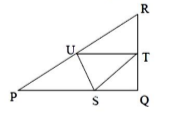
\includegraphics[width=0.7\textwidth]{Screenshot_2025_0816_191824.png}
	    \caption{}
    \label{fig:Q8}
    \end{figure}

    \hfill(GATE MN 2015)

\item Right triangle PQR is to be constructed in the xy-plane so that the right angle is at P and line PR is parallel to the x-axis. The x and y coordinates of P, Q, and R are to be integers that satisfy the inequalities:  
$-4 \leq x \leq 5$ and $6 \leq y \leq 16$.  

How many different triangles could be constructed with these properties?  

\hfill(GATE MN 2015)

\begin{enumerate}
		\begin{multicols}{4}
\item 110  
\item 1,100  
\item 9,900  
\item 10,000 
\end{multicols}
\end{enumerate}

\item A coin is tossed thrice. Let $X$ be the event that head occurs in each of the first two tosses.  
Let $Y$ be the event that a tail occurs on the third toss.  
Let $Z$ be the event that two tails occur in three tosses.  

Based on the above information, which one of the following statements is TRUE?  

\hfill(GATE MN 2015)

\begin{enumerate}
\begin{multicols}{4}		
\item $X$ and $Y$ are not independent  
\item $Y$ and $Z$ are dependent  
\item $Y$ and $Z$ are independent  
\item $X$ and $Z$ are independent
\end{multicols}	
\end{enumerate}

\item Out of the support categories given for an underground coal mine, identify the `active support'.  

	\hfill(GATE MN 2015)
\begin{multicols}{2}
\begin{enumerate}
\item wire mesh  
\item shotcrete  
\item fully grouted roof bolt  
\item hydraulic prop  
\end{enumerate}
\end{multicols}


\item Massive sandstone in immediate roof delays the local fall in goaf of a coal mine. Under this condition, crushing of the pillars at outbye side is called  

	\hfill(GATE MN 2015)
\begin{multicols}{2}
\begin{enumerate}
\item coal bump  
\item overriding of pillars  
\item stiffening of pillars  
\item spalling of pillars  
\end{enumerate}
\end{multicols}

\item A back sight on a bench mark of RL 100.00 m on the floor of a tunnel is 3.25 m. The inverse staff reading on a roof station of the tunnel is 1.25 m. The RL of the roof station in m is \underline    {\hspace{2cm}}.  




\item The angle in degrees at which a ridge line intersects contours is  

	\hfill(GATE MN 2015)
\begin{multicols}{4}
\begin{enumerate}
\item 0  
\item 30  
\item 45  
\item 90  
\end{enumerate}
\end{multicols}

\item In a drum hoisting system through a vertical shaft, overwinding is prevented by  


	\hfill(GATE MN 2015)
\begin{enumerate}
\item Lilly controller  
\item detaching hook  
\item caliper brake  
\item safety catch  
\end{enumerate}


\item The temperature of a parcel of air decreases from 30.2$^\circ$C to 28.9$^\circ$C as it rises from an altitude of 20 m to 120 m. The lapse rate for the atmosphere is 

	\hfill(GATE MN 2015)
\begin{multicols}{4}
\begin{enumerate}
\item subadiabatic  
\item adiabatic  
\item superadiabatic  
\item transadiabatic  
\end{enumerate}
\end{multicols}

\item The excess pore pressure in backfill material in a cut-and-fill stope leads to  


	\hfill(GATE MN 2015)
\begin{enumerate}
\item reduction in strength of the wall rock  
\item enhancement of bearing strength of fill  
\item loss of shear resistance of fill  
\item prevention of progressive failure of crown pillar  
\end{enumerate}

\item The primary purpose of cut holes for blasting in an underground drivage is to  


	\hfill(GATE MN 2015)
\begin{enumerate}
\item provide additional face area  
\item have smooth surface after blasting  
\item prevent over-breakage  
\item reduce noise  
\end{enumerate}

\item In a triangle ABC, the bearings of the sides AB, BC, and CA are 60$^\circ$, 130$^\circ$, and 270$^\circ$ respectively. The interior angles A, B, and C in degrees respectively are 

	\hfill(GATE MN 2015)
\begin{multicols}{2}
\begin{enumerate}
\item 110, 40, 30  
\item 60, 110, 30  
\item 30, 40, 110  
\item 30, 110, 40  
\end{enumerate}
\end{multicols}

\item In a binomial distribution, the probability of success $p \to 0$ and number of trials $n \to \infty$ such that $\lambda = np$ approaches to a finite value. The variance of the distribution is 

	\hfill(GATE MN 2015)
\begin{multicols}{4}
\begin{enumerate}
\item $np\lambda$  
\item $n\lambda$  
\item $p\lambda$  
\item $\lambda$  
\end{enumerate}
\end{multicols}

\item For a function $f(x)$, it is given that $f(0)=2$ and $f''(0)=4$. Ignoring all other higher order derivative terms, the value of $f(0.5)$ is \underline{\hspace{2cm}}.  

	\hfill(GATE MN 2015)


\item The two sides of a parallelogram are given by the vectors $\vec{A} = 2\hat{i} - 3\hat{j}$ and $\vec{B} = 3\hat{i} + 2\hat{j}$. The area of the parallelogram is  

	\hfill(GATE MN 2015)
\begin{multicols}{4}
\begin{enumerate}
\item 13  
\item 12  
\item 10  
\item 5  
\end{enumerate}
\end{multicols}

\item In a BOD test, 5 ml of wastewater is diluted with pure water to fill a 300 ml BOD bottle. The initial and final dissolved oxygen contents of the mix are 9.0 mg/l and 7.0 mg/l respectively. The BOD of the wastewater, in mg/l, is  

	\hfill(GATE MN 2015)
\begin{multicols}{4}
\begin{enumerate}
\item 2  
\item 10  
\item 120  
\item 600  
\end{enumerate}
\end{multicols}

\item A force of 50 N is applied to a wrench as shown in the figure.  
	The magnitude of the moment in N-mm of this force about the point P is \underline{\hspace{2cm}}.  
\begin{figure}[H]                                
\centering                            
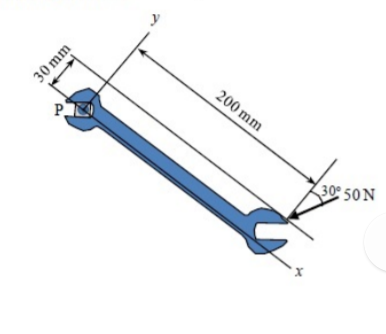
\includegraphics[width=0.7\textwidth]{Screenshot_2025_0817_211140.png}       
\caption{}      
\label{fig:Q8}          
\end{figure}


\hfill(GATE MN 2015)

\item Dilatancy of rock is associated with  

	\hfill(GATE MN 2015)

\begin{enumerate}
\item increase in surface area after fragmentation  
\item decrease in volume due to compression of rock  
\item increase in shear strain due to cracking of rock  
\item increase in volume due to cracking of rock  
\end{enumerate}


\item A bord and pillar panel having square pillars is designed for 30\% extraction during development. If the gallery width is 5 m, the side of the pillar in m is \underline{\hspace{2cm}}.  

	\hfill(GATE MN 2015)


\item Low shock and high gas pressure explosive is generally used for blasting of 

	\hfill(GATE MN 2015)
\begin{multicols}{2}
\begin{enumerate}
\item hard and brittle rock mass  
\item soft and jointed rock mass  
\item hard and massive intact rock mass  
\item soft and massive intact rock mass  
\end{enumerate}
\end{multicols}

\item The covariance of copper grade for a certain lag distance in an ore body is $6.0 \, (\%)^2$.  
If the sill is $10 \, (\%)^2$, the semivariogram for the same lag distance in $(\%)^2$ is 

\hfill(GATE MN 2015)
\begin{multicols}{4}
\begin{enumerate}
\item 4.0  
\item 16.0  
\item 2.0  
\item 64.0  
\end{enumerate}
\end{multicols}

\item The matrix  
\[
	\vec{A}=\myvec{
-4/6 & 2/6 & 4/6 \\
2/6 & -4/6 & 2/6 \\
2/6 & 4/6 & 4/6
}
\]
is  

\hfill(GATE MN 2015)
\begin{multicols}{4}
\begin{enumerate}
\item orthogonal  
\item diagonal  
\item skew-symmetric  
\item symmetric  
\end{enumerate}
\end{multicols}

\item A gas mixture contains CH$_4$, C$_2$H$_6$ and H$_2$ with respective concentrations of 75\%, 15\% and 10\% by volume. The lower explosibility limit of CH$_4$, C$_2$H$_6$ and H$_2$ are 5.0\%, 3.3\% and 4.2\% respectively.  
The lower explosibility limit of the gas mixture, in percentage, is \underline{\hspace{2cm}}.  

\hfill(GATE MN 2015)


\item Intake air containing 0.2\% methane enters a section of an underground mine where emission rate of methane is 0.05 m$^3$/s. Assuming that the threshold limit value of methane is 1.25\%, the minimum quantity of fresh air required in m$^3$/s is \underline{\hspace{2cm}}.  

	\hfill(GATE MN 2015)

\item In a fully mechanised bord and pillar mining system, winning of coal and its transportation from the face is commonly carried out with the combination of  

	\hfill(GATE MN 2015)

\begin{enumerate}
\item continuous miner, shuttle car, feeder breaker and belt conveyor  
\item continuous miner, LHD, feeder breaker and chain conveyor  
\item continuous miner, SDL, feeder breaker and belt conveyor  
\item continuous miner, shuttle car, feeder breaker and chain conveyor  
\end{enumerate}


\item An underground coal mine employing 1200 persons experiences 2 fatal injuries, 6 serious injuries and 8 reportable injuries during the year 2013. The total injury rate per 1000 persons employed for the year is \underline{\hspace{2cm}}.  

	\hfill(GATE MN 2015)

\item In self-contained chemical-oxygen self-rescuer, oxygen is produced by  
\begin{multicols}{4}
\begin{enumerate}
\item Hopcalite  
\item potassium peroxide  
\item sodium hydroxide  
\item Protosorb  
\end{enumerate}
\end{multicols}

\item The failure data of an equipment follows an exponential distribution. If the mean time between failures is 3000 hours, the reliability of the equipment for 750 hours is \underline{\hspace{2cm}}.

	\hfill(GATE MN 2015)


\item In a 4.2 m wide and 3.0 m high gallery in a coal seam, twelve shot holes are blasted per round. The holes are charged with 2 explosive cartridges of 435 g each. If the powder factor of the blast is 2.2 tonne/kg and specific gravity of coal is 1.4, the pull per round of blast in m is  

	\hfill(GATE MN 2015)
\begin{multicols}{4}
\begin{enumerate}
\item 1.45  
\item 1.70  
\item 1.30  
\item 4.06  
\end{enumerate}
\end{multicols}

\item The stadia readings with horizontal sight on a vertical staff held at 50 m from a tacheometer are 1.285 m and 1.780 m. The focal length of the object glass is 25 cm, and the distance between the object glass and the vertical axis of the tacheometer is 15 cm. The stadia interval in mm is \underline{\hspace{2cm}}.  


	\hfill(GATE MN 2015)

\item In a shortwall panel, coal is extracted from the face by a continuous miner having rate of production 30 tonne/h. Coal having specific gravity of 1.4 is transported by shuttle cars of capacity 0.9 m$^3$ each to a feeder breaker located at 60 m from the face. If the average speed of the LHD is 0.5 m/s, and total loading and unloading time of LHD is 40 s, the number of LHDs required to match the production of the continuous miner is  

	\hfill(GATE MN 2015)
\begin{multicols}{4}
\begin{enumerate}
\item 1  
\item 2  
\item 3  
\item 4  
\end{enumerate}
\end{multicols}

\item Vertical photographs of an area lying 500 m above the mean sea level are to be taken at a scale of 1:20000 from an aircraft. If the camera has a focal length of 210 mm, the flying height of the aircraft above the mean sea level in m is \underline{\hspace{2cm}}.  

	\hfill(GATE MN 2015)


\item Match the following locations with support types in coal mines.  

\begin{table}[H]                                 
\centering\normalsize
\begin{tabular}{ll}
\textbf{Location} & \textbf{ Support type}\\
P. Roadway junctions & 1. Powered support \\
Q. Between adjacent panels & 2. Chock and bolt \\
R. Longwall face & 3. Back fill \\
S. Goaf & 4. Barrier pillar \\
\end{tabular}
\caption{}
    \label{tab:Q40}
\end{table}

\hfill(GATE MN 2015)

\begin{multicols}{2}
\begin{enumerate}
\item P-2, Q-3, R-1, S-4  
\item P-4, Q-3, R-1, S-2  
\item P-2, Q-4, R-1, S-3  
\item P-2, Q-3, R-4, S-1  
\end{enumerate}
\end{multicols}

\item The value of 
\[
\int_{0}^{4} \sqrt{16 - x^2} \, dx
\] 
is  

\hfill(GATE MN 2015)
\begin{multicols}{4}
\begin{enumerate}
\item 12.57  
\item 50.24  
\item 25.12  
\item 3.14  
\end{enumerate}
\end{multicols}

\item A rectangular field of area 20000 m$^2$ is to be divided into 6 different plots by fencing as shown in the figure. The value of $L$ in m for which the total length of fencing becomes minimum is \underline{\hspace{2cm}}. 
\begin{figure}[H]                       
\centering            
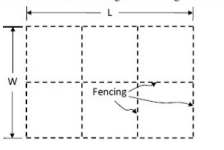
\includegraphics[width=0.7\textwidth]{Screenshot_2025_0817_214014.png}        
\caption{}          
\label{fig:Q42}   
\end{figure}

\hfill(GATE MN 2015)

\item Match the following for a drilling system.  


\begin{table}[H]
    \centering\normalsize
\begin{tabular}{ll}
	\textbf{Component } & \textbf{Function}\\
P. Drill & 1. Utilization of energy in fragmenting rock \\
Q. Drill rod & 2. Reduction of energy loss due to regrinding \\
R. Drill bit & 3. Conversion of original form of energy into mechanical energy \\
S. Flushing medium & 4. Transmission of energy from prime mover to applicator \\
\end{tabular}
\caption{}
    \label{tab:Q43}
\end{table}

\hfill(GATE MN 2015)

\begin{multicols}{2}
\begin{enumerate}
\item P-3, Q-1, R-2, S-4  
\item P-4, Q-1, R-3, S-2  
\item P-3, Q-4, R-1, S-2  
\item P-2, Q-1, R-3, S-4  
\end{enumerate}
\end{multicols}

\item For the ventilation system shown, the combined resistance of the trunk airways and the shafts is 2.2 Ns$^2$/m$^8$. The resistances of splits A and B are 0.5 Ns$^2$/m$^8$ and 0.8 Ns$^2$/m$^8$ respectively. A regulator of size 2.0 m$^2$ is placed in split A. Considering the fan generates a pressure of 1000 Pa, the air flow in m$^3$/s in split B is \underline{\hspace{2cm}}.  
\begin{figure}[H]                             
\centering                          
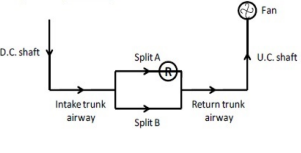
\includegraphics[width=0.7\textwidth]{Screenshot_2025_0817_212807.png}    
	\caption{}          
	\label{fig:Q44}        
\end{figure}

\hfill(GATE MN 2015)

\item A mine fan running at 300 rpm delivers 150 m$^{3}$/s of air at a pressure of 900 Pa. Fan and motor efficiencies are 75\% and 90\% respectively. If the fan speed is reduced to 250 rpm, the saving in electric power input to the motor in kW is \underline{\hspace{2cm}}.  

	\hfill(GATE MN 2015)

\item Subsidence profile function, $s(x)$, along the lateral cross-section over a flat longwall panel is given as  
\[
s(x) = 0.8 \Big[0.996 - \tanh\Big(\frac{8.3x}{D}\Big)\Big] \, \text{m}
\]  
where $x =$ distance (m) from the inflection point and $D =$ depth (m) of the seam. Considering that the inflection point lies vertically above the edge of the panel, the angle of draw in degrees for a depth of 250 m is \underline{\hspace{2cm}}. 

\hfill(GATE MN 2015)


\item A goaf void of 250 m$^{3}$ is filled in 3 hours by hydraulic sand stowing method. Density of the sand is 2.6 tonne/m$^{3}$. If the filling factor of goaf void is 0.9 and sand to water ratio in the stowing mixture is 1.0 tonne to 1.1 m$^{3}$, the stowing rate in m$^{3}$/h is \underline{\hspace{2cm}}.  


	\hfill(GATE MN 2015)

\item A single-acting reciprocating pump delivers 0.018 m$^{3}$/s of water when running at 45 cycles per minute. The piston diameter is 300 mm and stroke length is 400 mm. The volumetric efficiency of the pump in \% is \underline{\hspace{2cm}}. 

	\hfill(GATE MN 2015)


\item Match the method of mining with strength of orebody, type of support and orebody geometry.  


\begin{table}[H]
    \centering\normalsize
	\begin{tabular}{cccc}
		\textbf{Strength} &\textbf{Support} & \textbf{Geometry}& \textbf{Method}\\
 P. Strong & L. Unsupported & X. Tabular and steep & 1. Cut-and-fill \\
Q. Moderate &  M. Artificially supported    &  Y. Tabular and flat  & 2. Block caving \\
 R. Weak& N. Self-supporting  & Z. Massive and steep & 3. Room and Pillar \\

\end{tabular}
\caption{}
    \label{tab:Q49}
\end{table}

\hfill(GATE MN 2015)
\begin{enumerate}
\item P-N-X-3, Q-N-Z-2, R-L-Y-1  
\item P-L-X-1, Q-N-Z-3, R-M-Y-2  
\item P-N-Y-3, Q-M-X-1, R-L-Z-2  
\item P-L-Z-1, Q-N-Y-3, R-M-X-2  
\end{enumerate}


\item A mine air sample contains CH$_4$, CO, H$_2$, N$_2$ and O$_2$. The mine air analysis using Haldane apparatus gives the following results expressed in percentage of total sample volume.  
\begin{table}[H]                                   \centering\normalsize
\begin{tabular}{l l}
Total contraction after combustion & : 10.0 \\
CO$_2$ formed after combustion & : 6.0 \\
O$_2$ consumed in combustion & : 9.5 \\
\end{tabular}                                 
\caption{}                                  
\label{tab:Q50}
\end{table}

The percentage of CH$_4$ in the sample analysed is \underline{\hspace{2cm}}.  

\hfill(GATE MN 2015)


\item The initial investment for a small scale mining project is Rs. 5.0 crore. Annual cash inflow for a life period of 4 years is given below.  
\begin{table}[H]                                
\centering\normalsize
\begin{tabular}{cc}

Year & Cash inflow (Rs. crore) \\
1 & 1.5 \\
2 & 2.0 \\
3 & 2.0 \\
4 & 1.5 \\

\end{tabular}                               
\caption{}                                
\label{tab:Q51}
\end{table}

The net present value of the project at an annual discount rate of 10\% in Rs. crore is \underline{\hspace{2cm}}. 

\hfill(GATE MN 2015)

\item Given the following linear programming problem,  

Maximise \[
z = 3x_1 + 4x_2
\]  
Subject to  
\[
2x_1 + x_2 \leq 6
\]
\[
2x_1 + 3x_2 \leq 9
\]
\[
x_1 \geq 0, \; x_2 \geq 0
\]

The corner point feasible solution in terms of $(x_1,x_2)$ is  


\hfill(GATE MN 2015)
\begin{multicols}{4}
\begin{enumerate}
\item (1.5, 0)  
\item (1.25, 1.5)  
\item (0.5, 1.0)  
\item (2.25, 1.5)  
\end{enumerate}
\end{multicols}


\item The 3-period torque-time diagram of a statically balanced hoist is shown in the figure.
\begin{figure}[H]                    
\centering          
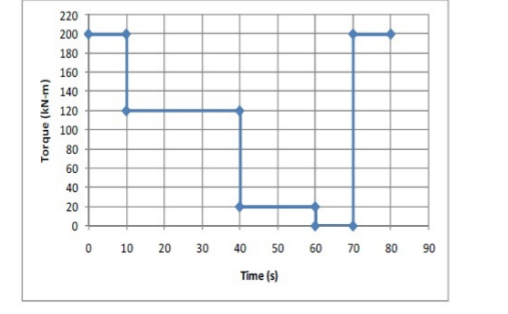
\includegraphics[width=0.7\textwidth]{Screenshot_2025_0818_083612.png}  
\caption{}   
\label{fig:Q53}
\end{figure}

The rms torque for the motor in kN-m is \underline{\hspace{2cm}}.

\hfill(GATE MN 2015)

\item Airborne PM$_{10}$ concentration in a residential area is monitored for 24 hours by a respirable dust sampler.  
Initial and final weights of the filter paper are 2.3125 g and 2.6996 g respectively.  
The average airflow rate during sampling is 1.2 m$^3$/min.  

The PM$_{10}$ concentration of the area in $\mu g/m^3$ is \underline{\hspace{2cm}}.  

\hfill(GATE MN 2015)


\item The assignment problem given requires four different jobs to be done on four different machines.  


\begin{table}[H]                                
\centering\normalsize
\begin{tabular}{|c|c|c|c|c|}
\hline
\multirow{2}{*}{Job} & \multicolumn{4}{c|}{Machine} \\ \cline{2-5}
 & $M_1$ & $M_2$ & $M_3$ & $M_4$ \\ \hline
$J_1$ & 27 & 35 & 36 & 30 \\ \hline
$J_2$ & 33 & 37 & 36 & 35 \\ \hline
$J_3$ & 30 & 26 & 28 & 24 \\ \hline
$J_4$ & 38 & 29 & 35 & 33 \\ \hline
\end{tabular}
\caption{}                                    
\label{tab:Q55}                          
\end{table}



The minimum cost of assignment is \underline{\hspace{2cm}}. 

\hfill(GATE MN 2015)

\item Acceleration of a particle moving in a straight line is expressed by  
\[
\frac{d^2 s}{dt^2} = 2t
\]  

where $s$ denotes distance (m) and $t$ time (s). At time $t=0$, the distance and velocity of the particle are 0 m and 3 m/s respectively.  

The distance travelled by the particle in m after 3 s is \underline{\hspace{2cm}}.

\hfill(GATE MN 2015)


\item Rock bolts have length $L = (150 + X)$ cm, where $X$ is a random variable with probability density function  

\[
f(x) = 
\begin{cases}
\dfrac{1}{4}(1 - 3x), & -2 \leq x \leq 2 \\
0, & \text{otherwise}
\end{cases}
\]

If 95\% of the bolt lengths ($L$) lie in the interval $150-c$ cm to $150+c$ cm, the value of $c$ is \underline{\hspace{2cm}}  

\hfill(GATE MN 2015)

  

\item The properties for a bivariate distribution of two random variables $X$ and $Y$ are given below.  

\[
E(X) = 24, \quad E(Y) = 36, \quad E(X^2) = 702, \quad E(Y^2) = 1524, \quad E(XY) = 1004
\]

The correlation coefficient between $X$ and $Y$ is \underline{\hspace{2cm}}  

\hfill(GATE MN 2015)


\item Biaxial stresses at a point inside a pillar are shown in the figure.  

\begin{figure}[H]                             
\centering
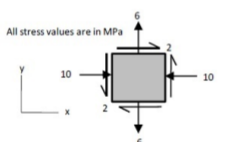
\includegraphics[width=0.35\textwidth]{Screenshot_2025_0818_084551.png} 
\caption{}                                    
\label{fig:Q59}                           
\end{figure}

The magnitude of the maximum shear stress in MPa and its direction with the x-axis in degrees at the same point respectively are  

\hfill(GATE MN 2015)

\begin{multicols}{2}
\begin{enumerate}
\item 8.25, 37.98  
\item 7.49, 37.98  
\item 8.25, 52.02  
\item 7.49, 52.02  
\end{enumerate}
\end{multicols}

 

\item A circular tunnel is constructed in a biaxial far field stress (vertical stress $p_0$ and horizontal stress $Kp_0$) as shown in the figure.  

\begin{figure}[H]                             
\centering
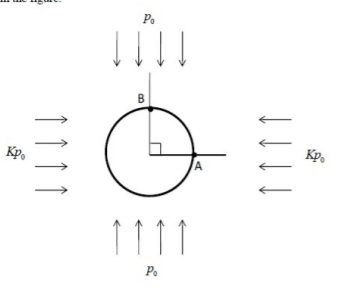
\includegraphics[width=0.35\textwidth]{Screenshot_2025_0818_084354.png} 
\caption{}                                      
\label{fig:Q60}                            
\end{figure}

If the ratio of the tangential stress measured at the boundary points A and B is 3:1, the value of $K$ is \underline{\hspace{2cm}}  

\hfill(GATE MN 2015)



\item Peak particle velocity (PPV) at points A and B are measured for a blast pattern as shown in the figure. \\

\begin{figure}[H]                                
\centering
	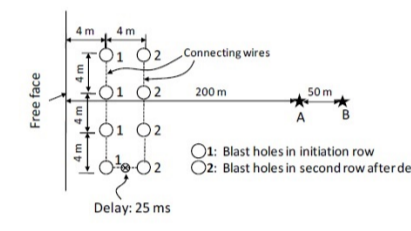
\includegraphics[width=0.8\textwidth]{Screenshot_2025_0818_085913.png}
\caption{}                                   
\label{fig:Q61}                          
\end{figure}

The relevant data are:
\begin{itemize}
\item Amount of explosives per hole in the 1st row : 500 kg
\item Amount of explosives per hole in the 2nd row : 475 kg
\item PPV at point A : 18 mm/s
\item PPV at point B : 10 mm/s
\end{itemize}

Considering the following relationship:
\[
PPV = K \left( \frac{D}{\sqrt{Q}} \right)^{-n}, \quad \text{mm/s}
\]

where \(D\) (in m) denotes the distance from the blast row to the measuring point and \(Q\) (in kg) the maximum charge per delay. The site constants \(K\) and \(n\) respectively are:

\hfill(GATE MN 2015)
\begin{multicols}{2}
\begin{enumerate}
\item 1002, 3.13
\item 622, 2.92
\item 823, 2.59
\item 1245, 2.99
\end{enumerate}
\end{multicols}


\item Copper ore of average grade 0.65\% is mined, milled, smelted and then refined. The following information is available:

\begin{itemize}
\item Mill recovery rate : 85\%
\item Average grade in mill concentrate : 20\%
\item Loss in smelting process : 5 kg/tonne of concentrate
\item Loss in refining process : 2 kg/tonne of blister copper
\end{itemize}

The amount of refined copper obtained per tonne of ore in kg is:

\hfill(GATE MN 2015)

\begin{multicols}{4}
\begin{enumerate}
\item 5.10
\item 5.37
\item 5.52
\item 6.50
\end{enumerate}
\end{multicols}


\item The ratio of horizontal to vertical in-situ stresses, \(K\), at a mine field varies with depth, \(D\) (in m) as
\[
K = \frac{267}{D} + 1.25
\]

If the unit weight of overburden rock is 25 kN/m$^3$, the horizontal stress in MPa at a depth of 400 m is \underline{\hspace{2cm}}.


\hfill(GATE MN 2015)

\item A coal seam of 2 m thickness is extracted by a longwall retreating panel with face length of 120 m. Web depth of the shearer is 0.6 m. Average manpower in the longwall face in a shift is 20. The specific gravity of in-situ coal is 1.4. If the shearer makes 4 full-face cuts in 3 shifts, the face OMS in tonne is \underline{\hspace{2cm}}.

	\hfill(GATE MN 2015)


\item A loaded dumper of total mass 75 tonne, having wheel diameter 1250 mm, runs on a haul road which offers an average specific rolling resistance of 260 N/tonne. The engine develops an axle torque of 15 kN-m. The starting acceleration of the dumper in m/s$^2$ is \underline{\hspace{2cm}}.

	\hfill(GATE MN 2015)


\end{enumerate}
\begin{center}                                  
\huge{END OF QUESTION PAPER}               
\end{center}
\end{document}


